\chapter{Ergebnisse und Evaluation}
Das Ergebnis der fertigen Anwendung hat die Erwartungen des Ziels (siehe Abschnitt \ref{chp:Ziele}) erf�llt. Die Systemqualit�t wird durch eine Reihe von einigen Verbesserungen deutlich erh�rt. Um das Programm zu testen, wird die Arbeit mit $36$ Videos durchgef�hrt. Die Videos haben eine Framerate von 10 Frames pro Sekunde und die Aufl�sung von 1080x720. Um multiperspektivische Ergebnisse zu bekommen, werden die Testvideos in verschiedenen R�umen aufgenommen. Die Testvideos wurden eine nach einander ohne Pause getestet, deswegen ver�ndern sich die Bilder auch ganz stark wie bei Drehung der Kamera. Auf diesem Grund wird eine Abwechslung des Testvideos auch als eine Drehung der Kamera betrachtet. Im Allgemein kann das Programm die au�ergew�hnliche Situation einer Person genau erkennen und das Ziel der Arbeit erf�llen. Zur Visualisierung wird eine au�ergew�hnliche Situation mit einer gekreuzten Begrenzungsbox markiert, in der die Testperson ist. Die alle Testvideos wurden annotiert, in welchem Zeitraum eine au�ergew�hnliche Situation passiert ist. Das Programm kann alle au�ergew�hnlichen Situationen erkennen, in den die Testperson auf dem Boden liegt und sich nicht mehr in 15 Bilder bewegt. Die au�ergew�hnlichen Situationen wurden genau dann annotiert, wenn die Testperson anf�ngt, auf dem Boden zu liegen. Das Programm wird hier betrachtet, ob es die au�ergew�hnliche in einem Zeitraum statt Zeitpunkt richtig erkennen kann. Zum Beispiel wird eine abnormale Situation von Bild 100 bis 200 annotiert und unser System markiert diese Situation von Bild 120 bis 210. Dann ist das nicht 100\% richtig, aber die Erkennung von der abnormalen Situation von Bild 100 bis 200 ist akzeptierbar.\\

F�r Messung der Laufzeit wurden die Tests auf einem Rechner Intel-Core i5 2.60 GHz ausgef�hrt. Die Laufzeit wird mehrmals gemessen und f�r jedes Bild braucht das System eine durchschnittliche Zeit von 109 Millisekunden. Das bedeutet in eine Sekunde kann das System 10 Bilder mit Aufl�sung von 1280x720 Pixel bearbeiten. Damit wird auch unser zweites Ziel realisiert und das Programm ist eine Echtzeitanwendung zur Erkennung der au�ergew�hnlichen Situation. Die Abbildung \ref{fig:laufzeit} stellt eine Laufzeit von 1000 Bildern in graphisch dar.\\

\begin{figure}[H]
	\centering
	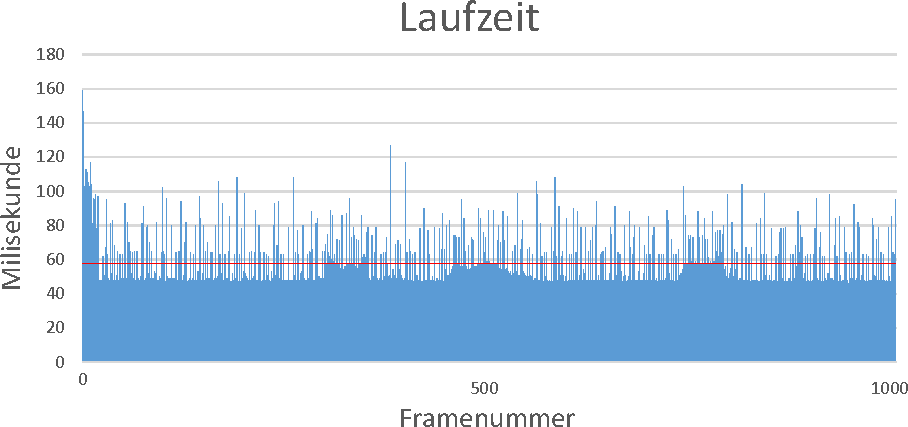
\includegraphics[width=1\textwidth]{fig/laufzeit.pdf}
	\caption{Laufzeit des Programms mit 1000 Bilder} 
	\label{fig:laufzeit}
\end{figure}

F�r die Darstellung der Ergebnisse wurden die Ergebnisse der verschiedenen Testvideos mit eine Abwechslung zwischen normalen und abnormalen Situationen analysiert und mit Graphik gezeigt. Auf der Abbildung \ref{fig:alarm} wurden die Ergebnisse des Programms mit den annotierten Musterergebnissen verglichen. Die gelbe Gerade geh�rt zu den erzeugten Ergebnisse und die blaue Gerade ist unser erwarteter Wert. Bei $0$ bedeutet ein Ausl�sen des Alarms, wobei es eine au�ergew�hnliche Situation erkannt ist. Bei $1$ wird nichts passiert, denn keine abnormale Situation erkannt ist. Unsere Ergebnisse sind nicht $100\%$ richtig von Bild nach Bild aber das Programm kann schon die Ereignisse in einem Zeitraum richtig erkennen. Die Ergebnisse liefert positive Werte zur�ck und die Anzahl der richtigen Erkennungen betragen immer h�her als $80\%$ der gesamten Bilder. Um das Programm zu bewerten, stellt die Abbildung \ref{fig:roc} eine ROC-Kurve von den Tests dar.

\begin{figure}[H]
	\centering
	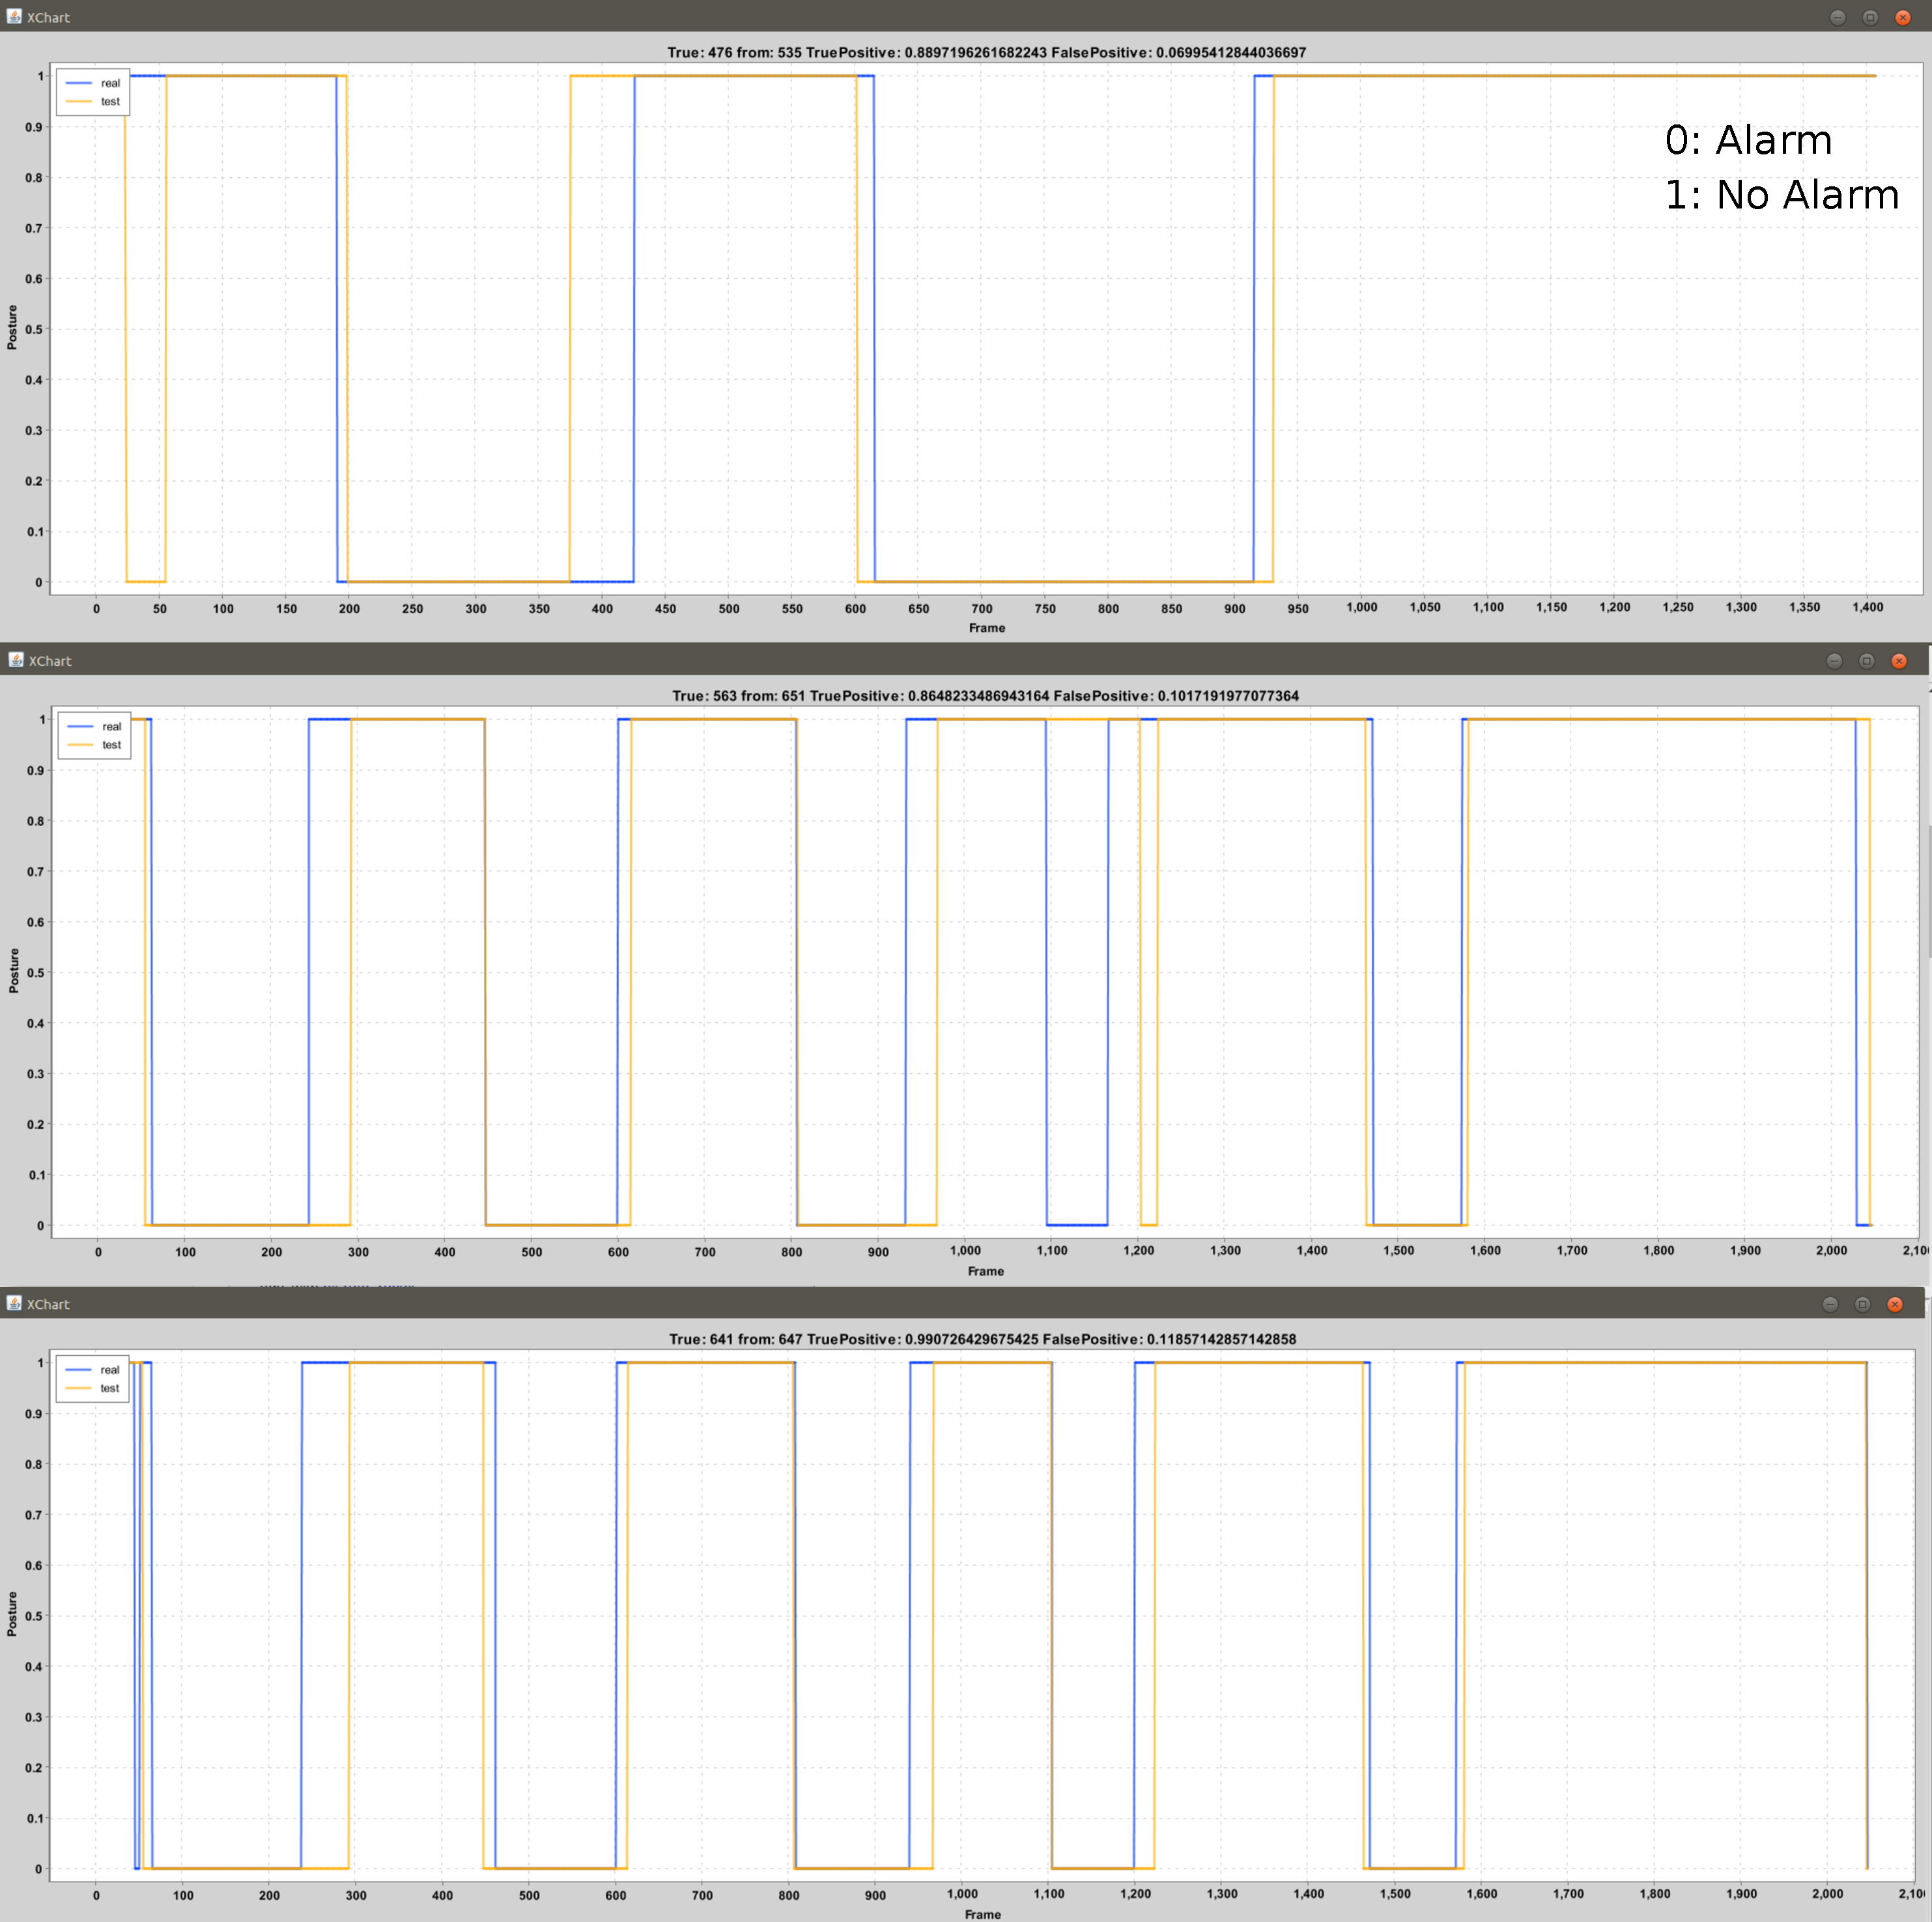
\includegraphics[width=1\textwidth]{fig/alarmevaluation.pdf}
	\caption{Die Ergebnisse aus der selbst aufgenommen Testvideos. Alle au�ergew�hnliche Situationen wurden mit der Anwendung richtig erkennen, } 
	\label{fig:alarm}
\end{figure}

\begin{figure}[H]
	\centering
	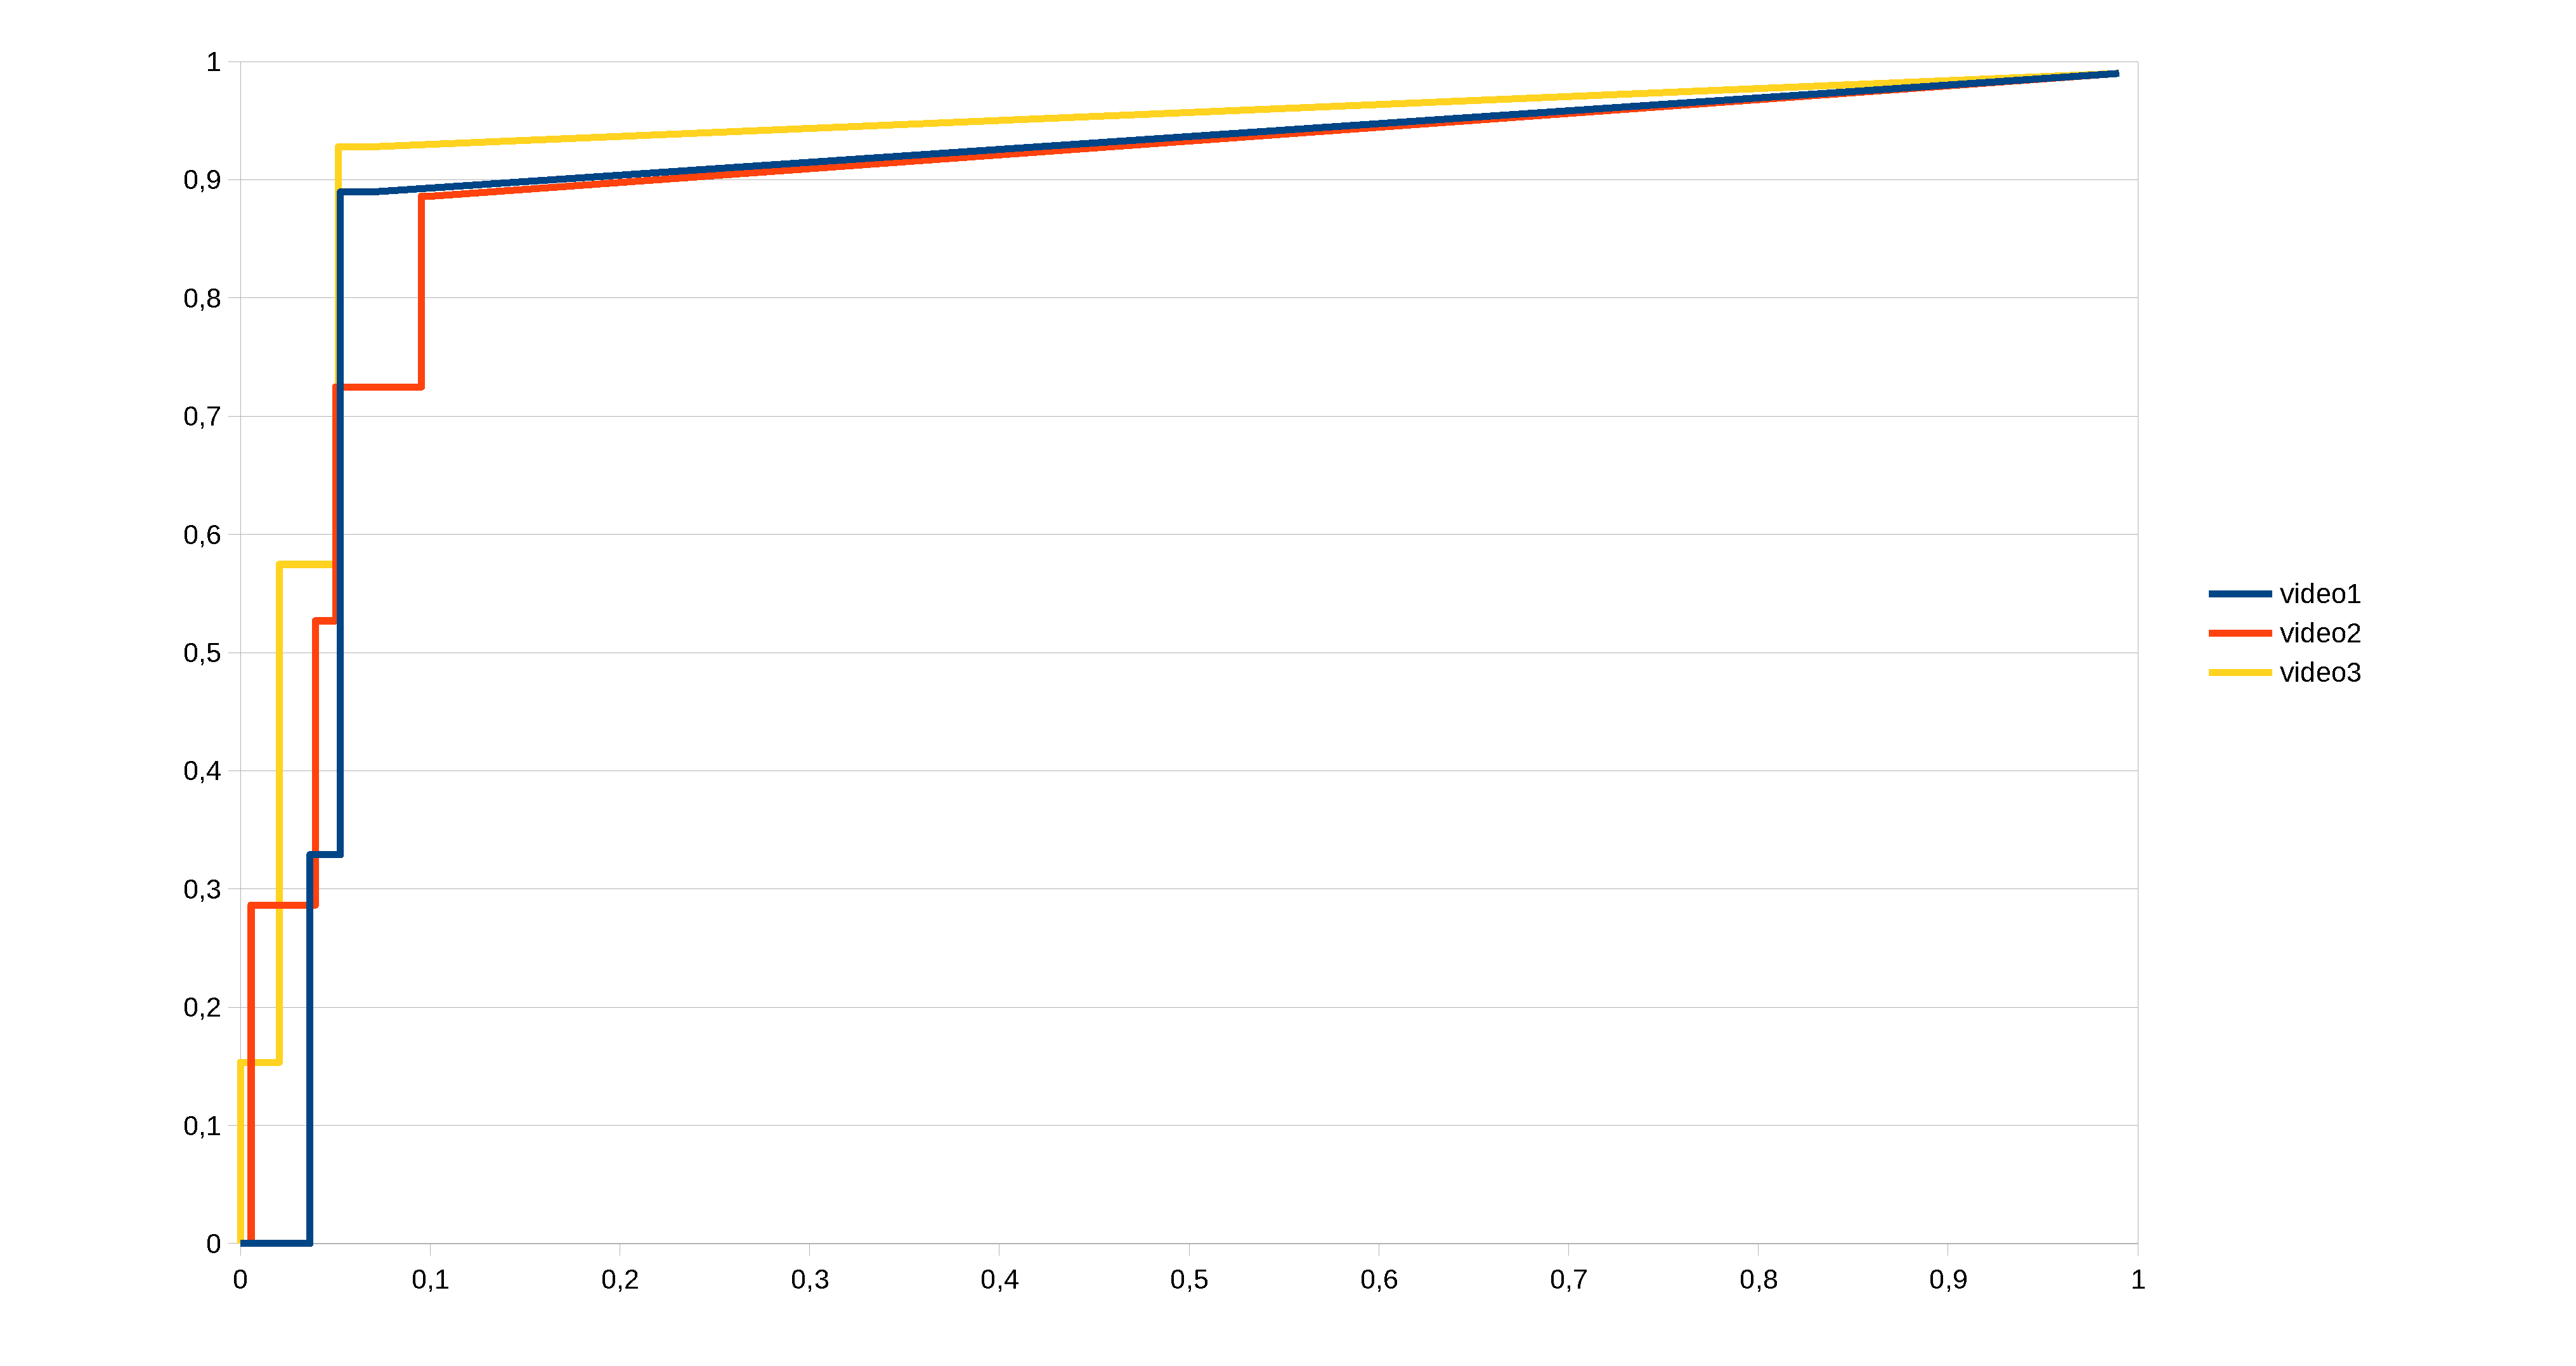
\includegraphics[width=1.1\textwidth]{fig/ROC.pdf}
	\caption{ROC-Kurze zur Bewertung des Programms.} 
	\label{fig:roc}
\end{figure}
